\PassOptionsToPackage{unicode=true}{hyperref} % options for packages loaded elsewhere
\PassOptionsToPackage{hyphens}{url}
%
\documentclass[]{article}
\usepackage{lmodern}
\usepackage{amssymb,amsmath}
\usepackage{ifxetex,ifluatex}
\usepackage{fixltx2e} % provides \textsubscript
\ifnum 0\ifxetex 1\fi\ifluatex 1\fi=0 % if pdftex
  \usepackage[T1]{fontenc}
  \usepackage[utf8]{inputenc}
  \usepackage{textcomp} % provides euro and other symbols
\else % if luatex or xelatex
  \usepackage{unicode-math}
  \defaultfontfeatures{Ligatures=TeX,Scale=MatchLowercase}
\fi
% use upquote if available, for straight quotes in verbatim environments
\IfFileExists{upquote.sty}{\usepackage{upquote}}{}
% use microtype if available
\IfFileExists{microtype.sty}{%
\usepackage[]{microtype}
\UseMicrotypeSet[protrusion]{basicmath} % disable protrusion for tt fonts
}{}
\IfFileExists{parskip.sty}{%
\usepackage{parskip}
}{% else
\setlength{\parindent}{0pt}
\setlength{\parskip}{6pt plus 2pt minus 1pt}
}
\usepackage{hyperref}
\hypersetup{
            pdftitle={Entregable: Algoritmos básicos de aprendizaje},
            pdfauthor={Laura Rodriguez Navas},
            pdfborder={0 0 0},
            breaklinks=true}
\urlstyle{same}  % don't use monospace font for urls
\usepackage[margin=1in]{geometry}
\usepackage{color}
\usepackage{fancyvrb}
\newcommand{\VerbBar}{|}
\newcommand{\VERB}{\Verb[commandchars=\\\{\}]}
\DefineVerbatimEnvironment{Highlighting}{Verbatim}{commandchars=\\\{\}}
% Add ',fontsize=\small' for more characters per line
\usepackage{framed}
\definecolor{shadecolor}{RGB}{248,248,248}
\newenvironment{Shaded}{\begin{snugshade}}{\end{snugshade}}
\newcommand{\AlertTok}[1]{\textcolor[rgb]{0.94,0.16,0.16}{#1}}
\newcommand{\AnnotationTok}[1]{\textcolor[rgb]{0.56,0.35,0.01}{\textbf{\textit{#1}}}}
\newcommand{\AttributeTok}[1]{\textcolor[rgb]{0.77,0.63,0.00}{#1}}
\newcommand{\BaseNTok}[1]{\textcolor[rgb]{0.00,0.00,0.81}{#1}}
\newcommand{\BuiltInTok}[1]{#1}
\newcommand{\CharTok}[1]{\textcolor[rgb]{0.31,0.60,0.02}{#1}}
\newcommand{\CommentTok}[1]{\textcolor[rgb]{0.56,0.35,0.01}{\textit{#1}}}
\newcommand{\CommentVarTok}[1]{\textcolor[rgb]{0.56,0.35,0.01}{\textbf{\textit{#1}}}}
\newcommand{\ConstantTok}[1]{\textcolor[rgb]{0.00,0.00,0.00}{#1}}
\newcommand{\ControlFlowTok}[1]{\textcolor[rgb]{0.13,0.29,0.53}{\textbf{#1}}}
\newcommand{\DataTypeTok}[1]{\textcolor[rgb]{0.13,0.29,0.53}{#1}}
\newcommand{\DecValTok}[1]{\textcolor[rgb]{0.00,0.00,0.81}{#1}}
\newcommand{\DocumentationTok}[1]{\textcolor[rgb]{0.56,0.35,0.01}{\textbf{\textit{#1}}}}
\newcommand{\ErrorTok}[1]{\textcolor[rgb]{0.64,0.00,0.00}{\textbf{#1}}}
\newcommand{\ExtensionTok}[1]{#1}
\newcommand{\FloatTok}[1]{\textcolor[rgb]{0.00,0.00,0.81}{#1}}
\newcommand{\FunctionTok}[1]{\textcolor[rgb]{0.00,0.00,0.00}{#1}}
\newcommand{\ImportTok}[1]{#1}
\newcommand{\InformationTok}[1]{\textcolor[rgb]{0.56,0.35,0.01}{\textbf{\textit{#1}}}}
\newcommand{\KeywordTok}[1]{\textcolor[rgb]{0.13,0.29,0.53}{\textbf{#1}}}
\newcommand{\NormalTok}[1]{#1}
\newcommand{\OperatorTok}[1]{\textcolor[rgb]{0.81,0.36,0.00}{\textbf{#1}}}
\newcommand{\OtherTok}[1]{\textcolor[rgb]{0.56,0.35,0.01}{#1}}
\newcommand{\PreprocessorTok}[1]{\textcolor[rgb]{0.56,0.35,0.01}{\textit{#1}}}
\newcommand{\RegionMarkerTok}[1]{#1}
\newcommand{\SpecialCharTok}[1]{\textcolor[rgb]{0.00,0.00,0.00}{#1}}
\newcommand{\SpecialStringTok}[1]{\textcolor[rgb]{0.31,0.60,0.02}{#1}}
\newcommand{\StringTok}[1]{\textcolor[rgb]{0.31,0.60,0.02}{#1}}
\newcommand{\VariableTok}[1]{\textcolor[rgb]{0.00,0.00,0.00}{#1}}
\newcommand{\VerbatimStringTok}[1]{\textcolor[rgb]{0.31,0.60,0.02}{#1}}
\newcommand{\WarningTok}[1]{\textcolor[rgb]{0.56,0.35,0.01}{\textbf{\textit{#1}}}}
\usepackage{graphicx,grffile}
\makeatletter
\def\maxwidth{\ifdim\Gin@nat@width>\linewidth\linewidth\else\Gin@nat@width\fi}
\def\maxheight{\ifdim\Gin@nat@height>\textheight\textheight\else\Gin@nat@height\fi}
\makeatother
% Scale images if necessary, so that they will not overflow the page
% margins by default, and it is still possible to overwrite the defaults
% using explicit options in \includegraphics[width, height, ...]{}
\setkeys{Gin}{width=\maxwidth,height=\maxheight,keepaspectratio}
\setlength{\emergencystretch}{3em}  % prevent overfull lines
\providecommand{\tightlist}{%
  \setlength{\itemsep}{0pt}\setlength{\parskip}{0pt}}
\setcounter{secnumdepth}{0}
% Redefines (sub)paragraphs to behave more like sections
\ifx\paragraph\undefined\else
\let\oldparagraph\paragraph
\renewcommand{\paragraph}[1]{\oldparagraph{#1}\mbox{}}
\fi
\ifx\subparagraph\undefined\else
\let\oldsubparagraph\subparagraph
\renewcommand{\subparagraph}[1]{\oldsubparagraph{#1}\mbox{}}
\fi

% set default figure placement to htbp
\makeatletter
\def\fps@figure{htbp}
\makeatother


\title{Entregable: Algoritmos básicos de aprendizaje}
\author{Laura Rodriguez Navas}
\date{Febrero 2020}

\begin{document}
\maketitle

\hypertarget{los-datos}{%
\subsection{Los Datos}\label{los-datos}}

El fichero glass.data incluye el estudio de la clasificación de los
tipos de vidrio con 6 variables explicativas. El estudio fue motivado
por una investigación criminológica. En la escena de un crimen, el
vidrio que queda puede usarse como evidencia \ldots{} ¡si se identifica
correctamente!

Las variables que se guardaron son:

\begin{enumerate}
\def\labelenumi{\arabic{enumi}.}
\tightlist
\item
  Id number: 1 to 214
\item
  RI: refractive index
\item
  Na: Sodium (unit measurement: weight percent in corresponding oxide,
  as are attributes 4-10)
\item
  Mg: Magnesium
\item
  Al: Aluminum
\item
  Si: Silicon
\item
  K: Potassium
\item
  Ca: Calcium
\item
  Ba: Barium
\item
  Fe: Iron
\item
  Type of glass: (class attribute)
\end{enumerate}

\begin{itemize}
\tightlist
\item
  1 building\_windows\_float\_processed
\item
  2 building\_windows\_non\_float\_processed
\item
  3 vehicle\_windows\_float\_processed
\item
  4 vehicle\_windows\_non\_float\_processed (none in this database)
\item
  5 containers
\item
  6 tableware
\item
  7 headlamps
\end{itemize}

Primero debemos cargar los datos como data frame, y le damos nombres a
las columnas.

\begin{Shaded}
\begin{Highlighting}[]
\NormalTok{glass <-}\StringTok{ }\KeywordTok{read.table}\NormalTok{(}\StringTok{"glass.data"}\NormalTok{, }\DataTypeTok{header =} \OtherTok{FALSE}\NormalTok{, }\DataTypeTok{sep =} \StringTok{","}\NormalTok{)}
\KeywordTok{names}\NormalTok{(glass) <-}\StringTok{ }\KeywordTok{c}\NormalTok{(}\StringTok{"Id number"}\NormalTok{, }\StringTok{"RI"}\NormalTok{, }\StringTok{"Na"}\NormalTok{, }\StringTok{"Mg"}\NormalTok{, }\StringTok{"Al"}\NormalTok{, }\StringTok{"Si"}\NormalTok{, }\StringTok{"K"}\NormalTok{, }\StringTok{"Ca"}\NormalTok{, }\StringTok{"Ba"}\NormalTok{, }\StringTok{"Fe"}\NormalTok{, }\StringTok{"Type of glass"}\NormalTok{)}
\KeywordTok{colnames}\NormalTok{(glass) <-}\StringTok{ }\KeywordTok{make.names}\NormalTok{(}\KeywordTok{colnames}\NormalTok{(glass))}
\KeywordTok{str}\NormalTok{(glass)}
\end{Highlighting}
\end{Shaded}

\begin{verbatim}
## 'data.frame':    214 obs. of  11 variables:
##  $ Id.number    : int  1 2 3 4 5 6 7 8 9 10 ...
##  $ RI           : num  1.52 1.52 1.52 1.52 1.52 ...
##  $ Na           : num  13.6 13.9 13.5 13.2 13.3 ...
##  $ Mg           : num  4.49 3.6 3.55 3.69 3.62 3.61 3.6 3.61 3.58 3.6 ...
##  $ Al           : num  1.1 1.36 1.54 1.29 1.24 1.62 1.14 1.05 1.37 1.36 ...
##  $ Si           : num  71.8 72.7 73 72.6 73.1 ...
##  $ K            : num  0.06 0.48 0.39 0.57 0.55 0.64 0.58 0.57 0.56 0.57 ...
##  $ Ca           : num  8.75 7.83 7.78 8.22 8.07 8.07 8.17 8.24 8.3 8.4 ...
##  $ Ba           : num  0 0 0 0 0 0 0 0 0 0 ...
##  $ Fe           : num  0 0 0 0 0 0.26 0 0 0 0.11 ...
##  $ Type.of.glass: int  1 1 1 1 1 1 1 1 1 1 ...
\end{verbatim}

Vemos como el conjunto de datos está formado por nueve variables
predictoras y la variable de classe Type.of.glass. Y todas las variables
són numéricas.

Además, podemos observar que la primera columna (cuyo nombre es
``Id.number'') es redundante (denota el identidficador de cada
instancia), por lo que borraremos esta columna. También le cambiaremos
el nombre a la última columna (cuyo nombre es ``Type.of.glass'') para
que se entienda mejor que respresenta la variable clase.

\begin{Shaded}
\begin{Highlighting}[]
\NormalTok{glass <-}\StringTok{ }\KeywordTok{subset}\NormalTok{(glass, }\DataTypeTok{select =} \OperatorTok{-}\NormalTok{Id.number)}
\KeywordTok{colnames}\NormalTok{(glass)[}\DecValTok{10}\NormalTok{] <-}\StringTok{ "Class"}
\KeywordTok{head}\NormalTok{(glass, }\DecValTok{10}\NormalTok{)}
\end{Highlighting}
\end{Shaded}

\begin{verbatim}
##         RI    Na   Mg   Al    Si    K   Ca Ba   Fe Class
## 1  1.52101 13.64 4.49 1.10 71.78 0.06 8.75  0 0.00     1
## 2  1.51761 13.89 3.60 1.36 72.73 0.48 7.83  0 0.00     1
## 3  1.51618 13.53 3.55 1.54 72.99 0.39 7.78  0 0.00     1
## 4  1.51766 13.21 3.69 1.29 72.61 0.57 8.22  0 0.00     1
## 5  1.51742 13.27 3.62 1.24 73.08 0.55 8.07  0 0.00     1
## 6  1.51596 12.79 3.61 1.62 72.97 0.64 8.07  0 0.26     1
## 7  1.51743 13.30 3.60 1.14 73.09 0.58 8.17  0 0.00     1
## 8  1.51756 13.15 3.61 1.05 73.24 0.57 8.24  0 0.00     1
## 9  1.51918 14.04 3.58 1.37 72.08 0.56 8.30  0 0.00     1
## 10 1.51755 13.00 3.60 1.36 72.99 0.57 8.40  0 0.11     1
\end{verbatim}

Aunque a primera vista los datos parecen que estan ordenados por la
variable clase Class, los ordenamos; y miramos que no existan valores
codificados como NA.

\begin{Shaded}
\begin{Highlighting}[]
\NormalTok{glass <-}\StringTok{ }\NormalTok{glass[}\KeywordTok{order}\NormalTok{(glass}\OperatorTok{$}\NormalTok{Class), ]}
\KeywordTok{any}\NormalTok{(}\KeywordTok{is.na}\NormalTok{(glass))}
\end{Highlighting}
\end{Shaded}

\begin{verbatim}
## [1] FALSE
\end{verbatim}

Como se ha comentado anteriormente, la columna Class representa la
variable clase. Concretamente en este estudio contamos con seis
variables explicativas.

A continuación, vamos a generar una representación binária. Primero, nos
quedaremos solo con los valores de la varible classe \{1, 2\}, los
renombraremos com \{1 = ``positive'', 2 = ``negative''\} y
factorizaremos.

\begin{Shaded}
\begin{Highlighting}[]
\NormalTok{glass <-}\StringTok{ }\KeywordTok{subset}\NormalTok{(glass , glass}\OperatorTok{$}\NormalTok{Class }\OperatorTok{<}\StringTok{ }\DecValTok{3}\NormalTok{)}
\ControlFlowTok{for}\NormalTok{ (i }\ControlFlowTok{in} \DecValTok{1}\OperatorTok{:}\DecValTok{146}\NormalTok{) \{}
  \ControlFlowTok{if}\NormalTok{ (glass}\OperatorTok{$}\NormalTok{Class[i] }\OperatorTok{==}\StringTok{ }\DecValTok{1}\NormalTok{)\{}
\NormalTok{    glass}\OperatorTok{$}\NormalTok{Class[i] <-}\StringTok{ 'positive'}
\NormalTok{  \}}
  \ControlFlowTok{else}\NormalTok{ \{}
\NormalTok{    glass}\OperatorTok{$}\NormalTok{Class[i] <-}\StringTok{ 'negative'}
\NormalTok{  \}}
\NormalTok{\}}
\NormalTok{glass[,}\DecValTok{10}\NormalTok{] <-}\StringTok{ }\KeywordTok{as.factor}\NormalTok{(glass[,}\DecValTok{10}\NormalTok{])}
\KeywordTok{str}\NormalTok{(glass)}
\end{Highlighting}
\end{Shaded}

\begin{verbatim}
## 'data.frame':    146 obs. of  10 variables:
##  $ RI   : num  1.52 1.52 1.52 1.52 1.52 ...
##  $ Na   : num  13.6 13.9 13.5 13.2 13.3 ...
##  $ Mg   : num  4.49 3.6 3.55 3.69 3.62 3.61 3.6 3.61 3.58 3.6 ...
##  $ Al   : num  1.1 1.36 1.54 1.29 1.24 1.62 1.14 1.05 1.37 1.36 ...
##  $ Si   : num  71.8 72.7 73 72.6 73.1 ...
##  $ K    : num  0.06 0.48 0.39 0.57 0.55 0.64 0.58 0.57 0.56 0.57 ...
##  $ Ca   : num  8.75 7.83 7.78 8.22 8.07 8.07 8.17 8.24 8.3 8.4 ...
##  $ Ba   : num  0 0 0 0 0 0 0 0 0 0 ...
##  $ Fe   : num  0 0 0 0 0 0.26 0 0 0 0.11 ...
##  $ Class: Factor w/ 2 levels "negative","positive": 2 2 2 2 2 2 2 2 2 2 ...
\end{verbatim}

La desición de quedarnos con los tipos de vidrio \{1, 2\} es porqué del
tipo de vidrio \{4\} no tenemos valores en este conjunto de datos para
clasificar, juntamente con el tipo de vidrio \{3\}; y los \{5, 6, 7\} no
pueden generar una representación biária con los otros tipos de vidrio.

\hypertarget{divisiuxf3n-de-los-datos-en-muestra-de-entrenamiento-y-de-test}{%
\subsection{División de los datos en muestra de entrenamiento y de
test}\label{divisiuxf3n-de-los-datos-en-muestra-de-entrenamiento-y-de-test}}

Tomaremos una muestra del 70\% del conjunto de datos como entrenamiento
y el 30\% del mismo como un conjunto de datos de prueba.

La validación cruzada usada cinco veces con muestreo estratificado se
utilizá para dividir el conjunto de datos.

\begin{Shaded}
\begin{Highlighting}[]
\KeywordTok{set.seed}\NormalTok{(}\DecValTok{123}\NormalTok{)}
\NormalTok{inTraining <-}\StringTok{ }\KeywordTok{createDataPartition}\NormalTok{(glass}\OperatorTok{$}\NormalTok{Class, }\DataTypeTok{p =} \FloatTok{.7}\NormalTok{, }\DataTypeTok{list =} \OtherTok{FALSE}\NormalTok{)}
\NormalTok{training <-}\StringTok{ }\NormalTok{glass[ inTraining,]}
\NormalTok{testing  <-}\StringTok{ }\NormalTok{glass[}\OperatorTok{-}\NormalTok{inTraining,]}
\NormalTok{fitControl <-}\StringTok{ }\KeywordTok{trainControl}\NormalTok{(}\DataTypeTok{method =} \StringTok{"cv"}\NormalTok{, }
                           \DataTypeTok{number =} \DecValTok{5}\NormalTok{,}
                           \DataTypeTok{classProbs =} \OtherTok{FALSE}\NormalTok{)}
\KeywordTok{str}\NormalTok{(training)}
\end{Highlighting}
\end{Shaded}

\begin{verbatim}
## 'data.frame':    103 obs. of  10 variables:
##  $ RI   : num  1.52 1.52 1.52 1.52 1.52 ...
##  $ Na   : num  13.9 13.5 13.2 13.3 12.8 ...
##  $ Mg   : num  3.6 3.55 3.69 3.62 3.61 3.6 3.61 3.6 3.66 3.43 ...
##  $ Al   : num  1.36 1.54 1.29 1.24 1.62 1.14 1.05 1.36 1.27 1.4 ...
##  $ Si   : num  72.7 73 72.6 73.1 73 ...
##  $ K    : num  0.48 0.39 0.57 0.55 0.64 0.58 0.57 0.57 0.6 0.69 ...
##  $ Ca   : num  7.83 7.78 8.22 8.07 8.07 8.17 8.24 8.4 8.56 8.05 ...
##  $ Ba   : num  0 0 0 0 0 0 0 0 0 0 ...
##  $ Fe   : num  0 0 0 0 0.26 0 0 0.11 0 0.24 ...
##  $ Class: Factor w/ 2 levels "negative","positive": 2 2 2 2 2 2 2 2 2 2 ...
\end{verbatim}

\begin{Shaded}
\begin{Highlighting}[]
\KeywordTok{str}\NormalTok{(testing)}
\end{Highlighting}
\end{Shaded}

\begin{verbatim}
## 'data.frame':    43 obs. of  10 variables:
##  $ RI   : num  1.52 1.52 1.52 1.52 1.52 ...
##  $ Na   : num  13.6 14 12.7 13.9 13 ...
##  $ Mg   : num  4.49 3.58 3.46 3.73 3.54 3.48 3.48 3.45 3.53 3.48 ...
##  $ Al   : num  1.1 1.37 1.56 1.18 1.21 1.41 1.33 1.21 1.32 1.35 ...
##  $ Si   : num  71.8 72.1 73.2 72.1 73 ...
##  $ K    : num  0.06 0.56 0.67 0.06 0.65 0.59 0.56 0.56 0.51 0.64 ...
##  $ Ca   : num  8.75 8.3 8.09 8.89 8.53 8.43 8.43 8.57 8.78 8.68 ...
##  $ Ba   : num  0 0 0 0 0 0 0 0 0.11 0 ...
##  $ Fe   : num  0 0 0.24 0 0 0 0 0 0 0 ...
##  $ Class: Factor w/ 2 levels "negative","positive": 2 2 2 2 2 2 2 2 2 2 ...
\end{verbatim}

\hypertarget{entrenamiento-de-los-modelos-y-evaluaciuxf3n}{%
\subsection{Entrenamiento de los modelos y
evaluación}\label{entrenamiento-de-los-modelos-y-evaluaciuxf3n}}

Se utilizarán tres algoritmos de clasificación diferentes para entrenar,
OneR, kNN y Multilayer Perceptrón.

\begin{enumerate}
\def\labelenumi{\arabic{enumi}.}
\tightlist
\item
  OneR.
\end{enumerate}

\begin{Shaded}
\begin{Highlighting}[]
\NormalTok{oner <-}\StringTok{ }\KeywordTok{train}\NormalTok{(Class }\OperatorTok{~}\StringTok{ }\NormalTok{., }\DataTypeTok{data =}\NormalTok{ training, }\DataTypeTok{method =} \StringTok{"OneR"}\NormalTok{, }\DataTypeTok{trControl =}\NormalTok{ fitControl)}
\NormalTok{oner}
\end{Highlighting}
\end{Shaded}

\begin{verbatim}
## Single Rule Classification 
## 
## 103 samples
##   9 predictor
##   2 classes: 'negative', 'positive' 
## 
## No pre-processing
## Resampling: Cross-Validated (5 fold) 
## Summary of sample sizes: 83, 82, 82, 82, 83 
## Resampling results:
## 
##   Accuracy   Kappa   
##   0.8452381  0.688327
\end{verbatim}

\begin{Shaded}
\begin{Highlighting}[]
\NormalTok{onerPredict <-}\StringTok{ }\KeywordTok{predict}\NormalTok{(oner, }\DataTypeTok{newdata =}\NormalTok{ testing)}
\NormalTok{cm_oner <-}\StringTok{ }\KeywordTok{confusionMatrix}\NormalTok{(onerPredict, testing}\OperatorTok{$}\NormalTok{Class)}
\NormalTok{cm_oner}
\end{Highlighting}
\end{Shaded}

\begin{verbatim}
## Confusion Matrix and Statistics
## 
##           Reference
## Prediction negative positive
##   negative       18        7
##   positive        4       14
##                                           
##                Accuracy : 0.7442          
##                  95% CI : (0.5883, 0.8648)
##     No Information Rate : 0.5116          
##     P-Value [Acc > NIR] : 0.001574        
##                                           
##                   Kappa : 0.4864          
##                                           
##  Mcnemar's Test P-Value : 0.546494        
##                                           
##             Sensitivity : 0.8182          
##             Specificity : 0.6667          
##          Pos Pred Value : 0.7200          
##          Neg Pred Value : 0.7778          
##              Prevalence : 0.5116          
##          Detection Rate : 0.4186          
##    Detection Prevalence : 0.5814          
##       Balanced Accuracy : 0.7424          
##                                           
##        'Positive' Class : negative        
## 
\end{verbatim}

\begin{enumerate}
\def\labelenumi{\arabic{enumi}.}
\setcounter{enumi}{1}
\tightlist
\item
  kNN con k=1, k=3 y con peso por distancia (tres configuraciones en
  total).
\end{enumerate}

\begin{Shaded}
\begin{Highlighting}[]
\NormalTok{grid_knn <-}\StringTok{ }\KeywordTok{expand.grid}\NormalTok{(}\DataTypeTok{k =} \KeywordTok{seq}\NormalTok{(}\DecValTok{1}\NormalTok{, }\DecValTok{3}\NormalTok{))}
\NormalTok{knn <-}\StringTok{ }\KeywordTok{train}\NormalTok{(Class }\OperatorTok{~}\StringTok{ }\NormalTok{., }\DataTypeTok{data =}\NormalTok{ training, }\DataTypeTok{method =} \StringTok{"knn"}\NormalTok{, }\DataTypeTok{trControl =}\NormalTok{ fitControl, }\DataTypeTok{tuneGrid =}\NormalTok{ grid_knn)}
\NormalTok{knn}
\end{Highlighting}
\end{Shaded}

\begin{verbatim}
## k-Nearest Neighbors 
## 
## 103 samples
##   9 predictor
##   2 classes: 'negative', 'positive' 
## 
## No pre-processing
## Resampling: Cross-Validated (5 fold) 
## Summary of sample sizes: 83, 82, 82, 82, 83 
## Resampling results across tuning parameters:
## 
##   k  Accuracy   Kappa    
##   1  0.7852381  0.5701258
##   2  0.7657143  0.5325650
##   3  0.7361905  0.4718654
## 
## Accuracy was used to select the optimal model using the largest value.
## The final value used for the model was k = 1.
\end{verbatim}

\begin{Shaded}
\begin{Highlighting}[]
\NormalTok{knnPredict <-}\StringTok{ }\KeywordTok{predict}\NormalTok{(knn, }\DataTypeTok{newdata =}\NormalTok{ testing)}
\NormalTok{cm_knn <-}\StringTok{ }\KeywordTok{confusionMatrix}\NormalTok{(knnPredict, testing}\OperatorTok{$}\NormalTok{Class)}
\NormalTok{cm_knn}
\end{Highlighting}
\end{Shaded}

\begin{verbatim}
## Confusion Matrix and Statistics
## 
##           Reference
## Prediction negative positive
##   negative       16        2
##   positive        6       19
##                                          
##                Accuracy : 0.814          
##                  95% CI : (0.666, 0.9161)
##     No Information Rate : 0.5116         
##     P-Value [Acc > NIR] : 3.932e-05      
##                                          
##                   Kappa : 0.6293         
##                                          
##  Mcnemar's Test P-Value : 0.2888         
##                                          
##             Sensitivity : 0.7273         
##             Specificity : 0.9048         
##          Pos Pred Value : 0.8889         
##          Neg Pred Value : 0.7600         
##              Prevalence : 0.5116         
##          Detection Rate : 0.3721         
##    Detection Prevalence : 0.4186         
##       Balanced Accuracy : 0.8160         
##                                          
##        'Positive' Class : negative       
## 
\end{verbatim}

\begin{enumerate}
\def\labelenumi{\arabic{enumi}.}
\setcounter{enumi}{2}
\tightlist
\item
  Multilayer Perceptrón con una sola capa oculta y 3, 5, y 7 unidades
  ocultas en la misma (tres configuraciones en total).
\end{enumerate}

\begin{Shaded}
\begin{Highlighting}[]
\NormalTok{grid_mlp =}\StringTok{ }\KeywordTok{expand.grid}\NormalTok{(}\DataTypeTok{layer1 =} \DecValTok{3}\NormalTok{, }\DataTypeTok{layer2 =} \DecValTok{5}\NormalTok{, }\DataTypeTok{layer3 =} \DecValTok{7}\NormalTok{)}
\NormalTok{mlp <-}\StringTok{ }\KeywordTok{train}\NormalTok{(Class }\OperatorTok{~}\NormalTok{., }\DataTypeTok{data =}\NormalTok{ training,}
             \DataTypeTok{method =} \StringTok{"mlpML"}\NormalTok{,}
             \DataTypeTok{trControl =}\NormalTok{ fitControl,}
             \DataTypeTok{tuneGrid =}\NormalTok{ grid_mlp)}
\NormalTok{mlp}
\end{Highlighting}
\end{Shaded}

\begin{verbatim}
## Multi-Layer Perceptron, with multiple layers 
## 
## 103 samples
##   9 predictor
##   2 classes: 'negative', 'positive' 
## 
## No pre-processing
## Resampling: Cross-Validated (5 fold) 
## Summary of sample sizes: 82, 83, 82, 82, 83 
## Resampling results:
## 
##   Accuracy   Kappa
##   0.5242857  0    
## 
## Tuning parameter 'layer1' was held constant at a value of 3
## Tuning
##  parameter 'layer2' was held constant at a value of 5
## Tuning parameter
##  'layer3' was held constant at a value of 7
\end{verbatim}

\begin{Shaded}
\begin{Highlighting}[]
\NormalTok{mlpPredict <-}\StringTok{ }\KeywordTok{predict}\NormalTok{(mlp, }\DataTypeTok{newdata =}\NormalTok{ testing)}
\NormalTok{cm_mlp <-}\StringTok{ }\KeywordTok{confusionMatrix}\NormalTok{(mlpPredict,testing}\OperatorTok{$}\NormalTok{Class)}
\NormalTok{cm_mlp}
\end{Highlighting}
\end{Shaded}

\begin{verbatim}
## Confusion Matrix and Statistics
## 
##           Reference
## Prediction negative positive
##   negative       22       21
##   positive        0        0
##                                           
##                Accuracy : 0.5116          
##                  95% CI : (0.3546, 0.6669)
##     No Information Rate : 0.5116          
##     P-Value [Acc > NIR] : 0.561           
##                                           
##                   Kappa : 0               
##                                           
##  Mcnemar's Test P-Value : 1.275e-05       
##                                           
##             Sensitivity : 1.0000          
##             Specificity : 0.0000          
##          Pos Pred Value : 0.5116          
##          Neg Pred Value :    NaN          
##              Prevalence : 0.5116          
##          Detection Rate : 0.5116          
##    Detection Prevalence : 1.0000          
##       Balanced Accuracy : 0.5000          
##                                           
##        'Positive' Class : negative        
## 
\end{verbatim}

Las métricas más adecuadas para la clasificación son Accuracy y
F-measure (Sensitivity y Specificity)

Kappa 0?

Utilizando la información que nos dan las matrizes de confusion
contruimos una tabla con estas métricas.

TABLA

Análisis de la tabla. el accuray mayor contienen menos errores, es mejor
modelo.

F measure.

\hypertarget{anuxe1lisis-roc}{%
\subsection{Análisis ROC}\label{anuxe1lisis-roc}}

Para el análisis ROC volveremos a predecir, pero ahora con el conjunto
de datos de prueba y construiremos el objecto de prediccion para cada
modelo de classificación utilizando el vector de estimación de
probabilidadas para la variable classe positiva.

\begin{enumerate}
\def\labelenumi{\arabic{enumi}.}
\tightlist
\item
  OneR.
\end{enumerate}

\begin{Shaded}
\begin{Highlighting}[]
\NormalTok{onerPredictProb <-}\StringTok{ }\KeywordTok{predict}\NormalTok{(oner, }\DataTypeTok{newdata =}\NormalTok{ testing, }\DataTypeTok{type =} \StringTok{"prob"}\NormalTok{)}
\NormalTok{onerPred <-}\StringTok{ }\KeywordTok{prediction}\NormalTok{(onerPredictProb}\OperatorTok{$}\NormalTok{positive, testing}\OperatorTok{$}\NormalTok{Class)}
\NormalTok{onerPerf <-}\StringTok{ }\KeywordTok{performance}\NormalTok{(onerPred, }\StringTok{"tpr"}\NormalTok{, }\StringTok{"fpr"}\NormalTok{)}
\end{Highlighting}
\end{Shaded}

\begin{enumerate}
\def\labelenumi{\arabic{enumi}.}
\setcounter{enumi}{1}
\tightlist
\item
  kNN con k=1, k=3 y con peso por distancia (tres configuraciones en
  total).
\end{enumerate}

\begin{Shaded}
\begin{Highlighting}[]
\NormalTok{knnPredictProb <-}\StringTok{ }\KeywordTok{predict}\NormalTok{(knn, }\DataTypeTok{newdata =}\NormalTok{ testing, }\DataTypeTok{type =} \StringTok{"prob"}\NormalTok{)}
\NormalTok{knnPred <-}\StringTok{ }\KeywordTok{prediction}\NormalTok{(knnPredictProb}\OperatorTok{$}\NormalTok{positive, testing}\OperatorTok{$}\NormalTok{Class)}
\NormalTok{knnPerf <-}\StringTok{ }\KeywordTok{performance}\NormalTok{(knnPred, }\StringTok{"tpr"}\NormalTok{, }\StringTok{"fpr"}\NormalTok{)}
\end{Highlighting}
\end{Shaded}

\begin{enumerate}
\def\labelenumi{\arabic{enumi}.}
\setcounter{enumi}{2}
\tightlist
\item
  Multilayer Perceptrón con una sola capa oculta y 3, 5, y 7 unidades
  ocultas en la misma (tres configuraciones en total).
\end{enumerate}

\begin{Shaded}
\begin{Highlighting}[]
\NormalTok{mlpPredictProb <-}\StringTok{ }\KeywordTok{predict}\NormalTok{(mlp, }\DataTypeTok{newdata =}\NormalTok{ testing, }\DataTypeTok{type =} \StringTok{"prob"}\NormalTok{)}
\NormalTok{mlpPred <-}\StringTok{ }\KeywordTok{prediction}\NormalTok{(mlpPredictProb}\OperatorTok{$}\NormalTok{positive, testing}\OperatorTok{$}\NormalTok{Class)}
\NormalTok{mlpPerf <-}\StringTok{ }\KeywordTok{performance}\NormalTok{(mlpPred, }\StringTok{"tpr"}\NormalTok{, }\StringTok{"fpr"}\NormalTok{)}
\end{Highlighting}
\end{Shaded}

Dibujamos las curvas ROC de los modelos.

\begin{Shaded}
\begin{Highlighting}[]
\KeywordTok{plot}\NormalTok{(onerPerf, }\DataTypeTok{col =} \StringTok{"orange"}\NormalTok{, }\DataTypeTok{add =} \OtherTok{FALSE}\NormalTok{)}
\KeywordTok{plot}\NormalTok{(knnPerf, }\DataTypeTok{col =} \StringTok{"blue"}\NormalTok{, }\DataTypeTok{add =} \OtherTok{TRUE}\NormalTok{)}
\KeywordTok{plot}\NormalTok{(mlpPerf, }\DataTypeTok{col =} \StringTok{"black"}\NormalTok{, }\DataTypeTok{add =} \OtherTok{TRUE}\NormalTok{)}
\KeywordTok{title}\NormalTok{(}\DataTypeTok{main =} \StringTok{"CURVAS ROC"}\NormalTok{)}
\KeywordTok{legend}\NormalTok{(}\StringTok{"bottomright"}\NormalTok{, }\DataTypeTok{legend =} \KeywordTok{c}\NormalTok{(}\StringTok{"OnerR"}\NormalTok{, }\StringTok{"kNN"}\NormalTok{, }\StringTok{"MLP"}\NormalTok{), }\DataTypeTok{col =} \KeywordTok{c}\NormalTok{(}\StringTok{"orange"}\NormalTok{, }\StringTok{"blue"}\NormalTok{, }\StringTok{"black"}\NormalTok{), }\DataTypeTok{lty =} \DecValTok{1}\NormalTok{, }\DataTypeTok{lwd =} \DecValTok{1}\NormalTok{)}
\end{Highlighting}
\end{Shaded}

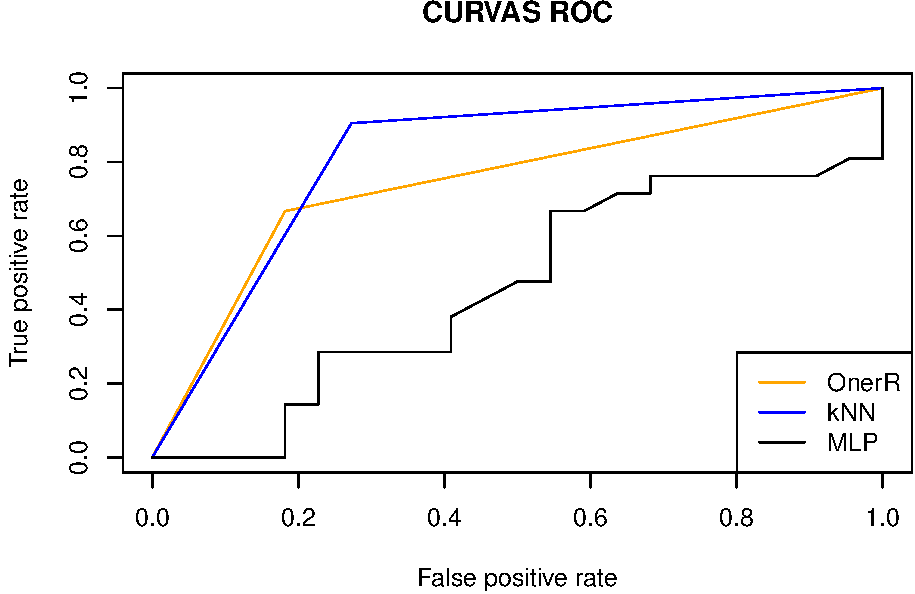
\includegraphics{document_files/figure-latex/unnamed-chunk-12-1.pdf}

Si nos fijamos en el gráfico de las curvas ROC que refleja el análisis
ROC podemos observar que el modelo de classificación k-Nearest Neighbors
para k=1 es el mejor para clasificar.

\end{document}
